\section{Considerações Finais}

Finalizando o procedimento, conectamos o ESP32 ao computador e enviamos o código para o microcontrolador utilizando o comando \textit{Alt + Ctrl + U} para que a extensão do Platform IO faça o envio. E para testar o sensor, usamos um telefone que se aproxima lentamente do sensor. As medidas no monitor vão diminuindo e as cores do LED RGB vão se alterando.

\begin{figure}[H]
    \centering
    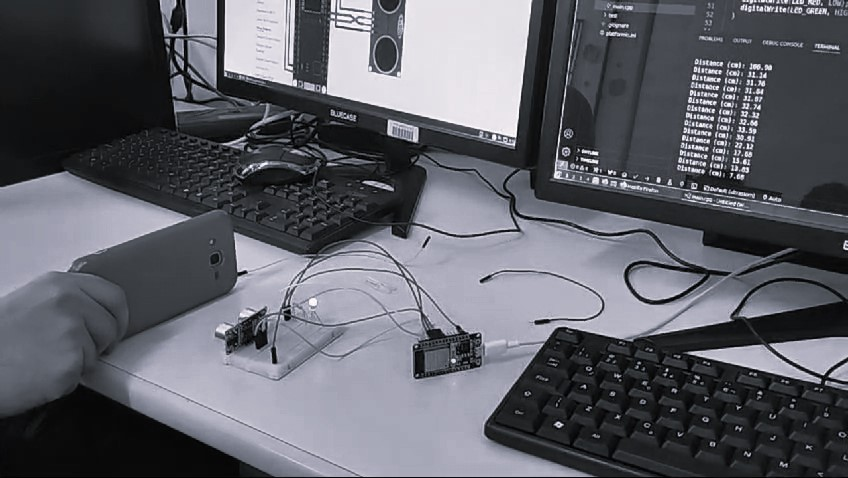
\includegraphics[width=0.5\linewidth]{img/teste.jpg}
    \caption{Resultado final.}
    \label{fig:result}
\end{figure}

Para conferir a execução da prática, é possível assistir esse \href{https://youtu.be/RUkX7DxMiUE}{vídeo} que foca em mostrar os dados no monitor, e nesse \href{https://youtu.be/0zt2-xrlvYo}{vídeo} que mostra o LED RGB mudando de cor conforme o objeto vai se aproximando do sensor. O código da prática pode ser visto nesse \href{https://github.com/fabricio-araujo94/microcontroladores/tree/main/ultrassom}{repositório} no GitHub.